% vim: set textwidth=78 autoindent:

\section{Complementos de QGIS}\label{sec:plugins}\index{plugins}

% when the revision of a section has been finalized, 
% comment out the following line:
%\updatedisclaimer

QGIS ha sido diseñado con una arquitectura de complementos.
Esto permite que nuevas características/funciones sean fácilmente añadidas a la aplicación.
Muchas de las características en QGIS están actualmente implementadas como complementos \textbf{del núcleo} o \textbf{externos}.\index{plugins!types} 

\begin{itemize}
\item \textbf{Complementos del núcleo} son implementados por el Equipo de Desarrollo de QGIS y son parte automáticamente de cada distribución de QGIS.
Están escritos en uno de dos lenguajes: C++ o Python.
Más información acerca de complementos del núcleo se provee en la sección \ref{sec:core_plugins}.
\item \textbf{Complementos Externos} actualmente todos escritos en Python.
Están almacenados en repositorios externos y son mantenidos por sus autores.
Pueden ser agregadas a QGIS usando el \filename{Plugin Installer}.
Mas información acerca de complementos externos se provee en la sección \ref{sec:external_plugins}.
\end{itemize}

\subsection{Administrando Complementos}\label{sec:managing_plugins}
\index{plugins!managing} 

Administrar complementos en general significa cargarlos o descargarlos usando el \filename{Administrador de complementos}.
Los complementos externos primero necesitan ser instalados usando el \filename{Instalador de Complementos}.

\subsubsection{Cargando un complemento del núcleo de de QGIS}\label{sec:load_core_plugin} 

La carga de un complemento del núcleo de QGIS se realiza desde el menú principal \mainmenuopt{Complementos} > \dropmenuopttwo{mActionShowPluginManager}{Administrar complementos...}.\index{plugins!manager}

\begin{figure}[ht]
   \begin{center}
   \caption{Administrador de Complementos \nixcaption}\label{fig:pluginmanager}\smallskip
   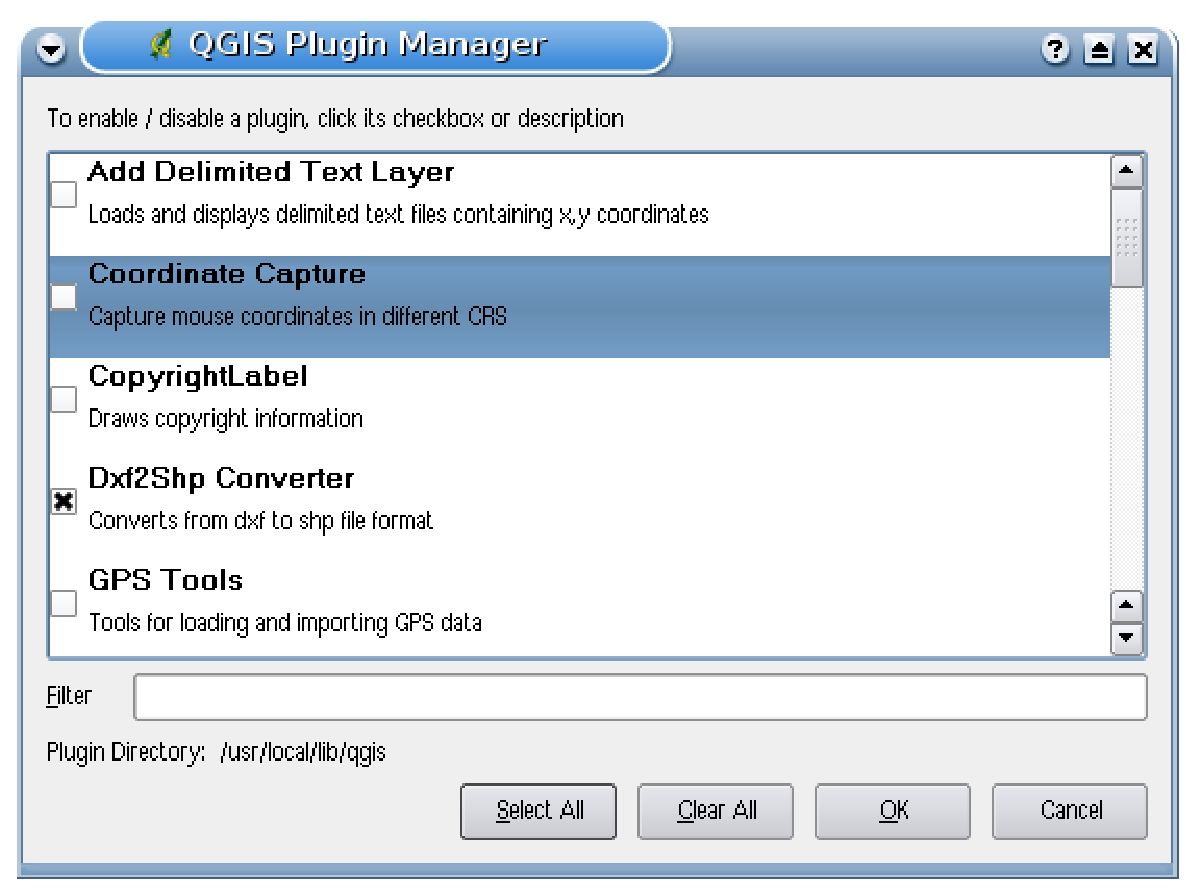
\includegraphics[clip=true, width=14cm]{pluginmanager}
\end{center}
\end{figure}

El \filename{Administrador de complementos} lista todos los complementos disponibles y su estado (cargado o descargado), 
incluyendo todos los complementos del núcleo y todos los complementos externos que han sido añadidos usando el \filename{Instalador de Complementos} 
(vea la sección \ref{sec:external_plugins}). Esos complementos que ya están cargados tiene un marca de verificación 
a la izquierda de su nombre. La figura \ref{fig:pluginmanager} muestra el diálogo de Administración de Complementos.

Para activar un complemento particular, haga clic en la caja de verificación a la izquierda del nombre del complemento, y clic \button{OK}. 
Cuando finalize la aplicación, una lista de los complementos cargados es retenida, y la próxima vez 
que ejecuta QGIS estos complementos son cargados automáticamente.

\begin{Tip}\caption{\textsc{Complementos defectuosos}}\index{crashes}
\qgistip{Si encuentra que QGIS falla al iniciar, un complemento puede estar fallando.
Puede parar todos los complementos de cargarse editando sus archivo de preferencias (vea \ref{subsec:gui_options} para su localización).
Localice las preferencias de complementos y cambie todos los valores de complementos a falso para prevenir que se carguen.
\nix {Por ejemplo, para evitar que el complemento de Texto Delimitado se cargue, la entrada en \$HOME/.config/QuantumGIS/qgis.conf en Linux debería verse así:\usertext{Add Delimited Text Layer=false}.}
\normalfont 
Haga esto para cada complemento en la sección [Plugins].
Entonces puede iniciar QGIS y agregar los complementos uno a la vez desde el \filename{Administrador de Complementos} para 
determinar cual complemento está causando el problema.}
\end{Tip} 

\subsubsection{Cargando complementos de QGIS externos}\label{sec:load_external_plugin} 

Hay dos pasos requeridos para integrar complementos externos a QGIS: 

\begin{enumerate}
\item Bajar un complementos externo desde un repositorio usando el \filename{Instalador de Complementos} (Sección \ref{sec:python_plugin_installer}).
El nuevo complemento externo será añadido a la lista de complementos disponibles en el \filename{Administrador de Complementos}.
\item Cargar el complemento usando el \filename{Administrador de Complementos}.
\end{enumerate}

\subsubsection{Usando el Instalador de Complementos Python de QGIS}\index{plugins!installing}\label{sec:python_plugin_installer}
\index{plugins!Python Plugin Installer}\index{plugins!upgrading}

\begin{figure}[ht]
   \begin{center}
   \caption{Instalando complementos python externos \nixcaption}
\label{fig:plugininstaller}\smallskip
   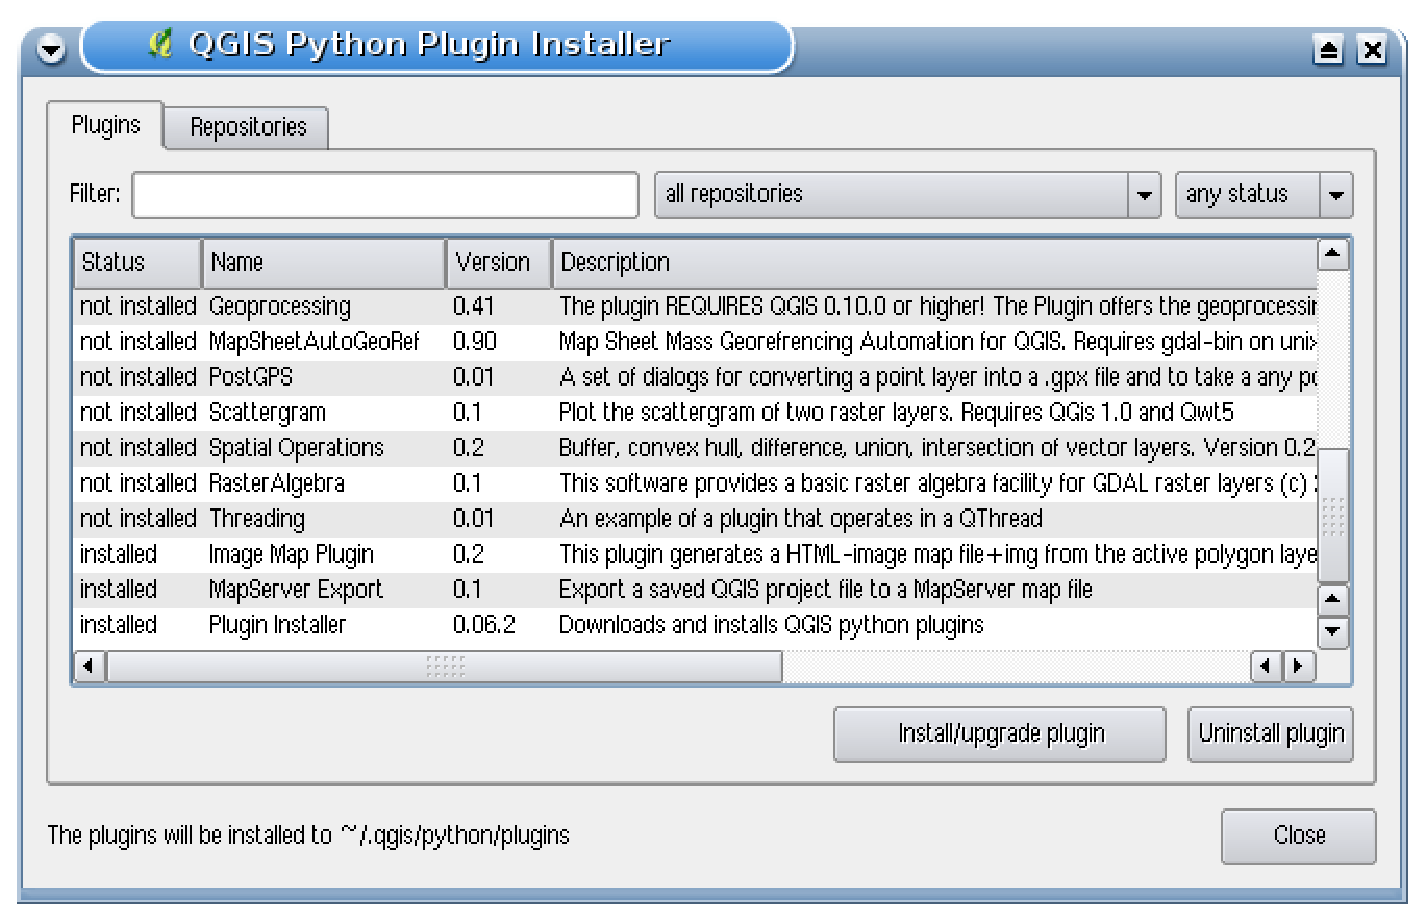
\includegraphics[clip=true, width=14cm]{plugininstaller}
\end{center}
\end{figure}

Para bajar e instalar un complementos externo de Python, haga clic en el menú \mainmenuopt{Complementos} > \dropmenuopttwo{plugin_installer}{Obtener Complementos de Python...}.
La ventana del \filename{Instalador de Complementos} aparecerá (figura \ref{fig:plugininstaller}) con la pestaña \tab{Complementos}, conteniendo una lista de todos los complementos de python instalados localmente, así como los complementos disponibles en repositorios remotos. Cada complementos puede estar:
\begin{itemize}
\item \textbf{no instalado} - esto significa que el complemento está disponible en el repositorio, pero no está instalado todavía. Para poder instalarlo, seleccione el complemento de la lista y haga clic en el botón \button{Instalar complemento}.
\item \textbf{nuevo} - esto significa que el complemento es nuevo en el repositorio.
\item \textbf{instalado} - esto indica que el complemento ha sido instalado. Si también está disponible en cualquier repositorio el botón \button{Reinstalar complemento} será activado. Si la versión disponible es mas vieja que la versión instalada, el botón \button{Downgrade complemento} aparecerá en su lugar.
\item \textbf{actualizable} - esto significa que el complemento está instalado, pero hay una versión actualizada disponible. en este caso, el  \button{Actualizar complemento} será activado.
\item \textbf{no válido} - esto significa que el complemento está instalado, pero no está disponible o roto. La razón se explicará en el campo de descripción del complemento.
\end{itemize}

\minisec{Pestaña complementos}

Para instalar un complemento, seleccionelo de la lista y haga clic en el botón \button{Instalar complemento}. El complemento es instalado en su propio directorio. 

\begin{itemize}
\item \nix{Linux y otros Unix}:\\
./share/qgis/python/plugins \\
/home/\$USERNAME/.qgis/python/plugins
\item \osx{Mac OS X}:\\
./Contents/MacOS/share/qgis/python/plugins \\
/Users/\$USERNAME/.qgis/python/plugins
\item \win{Windows}:\\
C:\textbackslash Program Files\textbackslash QGIS\textbackslash
python\textbackslash plugins \\
C:\textbackslash Documents and Settings\textbackslash\$USERNAME\textbackslash
.qgis\textbackslash python\textbackslash plugins
\end{itemize}

Si la instalación fue exitosa, un mensaje de confirmación aparecerá diciéndole  que vaya a  \mainmenuopt{Complementos} > \dropmenuopttwo{mActionShowPluginManager}{Administrar complementos...} para cargar el complemento recién instalado.

Si la instalación falla, la razón de la falla será mostrada en un diálogo de advertencia. Mas frecuentemente, los errores son el resultado de problemas de conexión y/o módulos de Python faltantes. En el primer caso necesitará esperar antes de tratar de instalar nuevamente, en el  segundo caso, debería de instalar los módulos faltantes relevantes a su sistemas operativo antes de usar el complemento. \nix{Para Linux, la mayoría de los módulos requeridos deberían estar disponibles via el administrador de paquetes}. \win{Para instrucciones de instalación en Windows visite la página del módulo}. Si está usando un proxy, necesitará configurarlo bajo \mainmenuopt{Editar} > \dropmenuopttwo{mActionOptions}{Opciones} (Gnome, OSX) 
or \mainmenuopt{Configuración} > \dropmenuopttwo{mActionOptions}{Opciones} (KDE, Windows) en la pestaña \tab{Proxy}.

El botón \button{Desinstalar complemento} está activo solo si el complemento seleccionado está instalado y no es un complemento del núcleo. Note que si ha instalado una actualización a un complemento del núcleo, puede desinstalar la actualización con el botón \button{Desinstalar complemento} y revertir a la versión entregada con Quantum GIS. La versión predeterminada sin embargo, no puede ser desinstalado.

\minisec{Pestaña Repositorios}

La segunda pestaña \tab{Repositorios}, contiene una lista de los repositorios de complementos disponibles para el \filename{Instalador de Complementos}. En forma predeterminada, solo el repositorio oficial de QGIS está activo. Puede agregar múltiples repositorios contribuidos por usuarios, incluyendo el repositorio contribuido central de QGIS y otros repositorios externos haciendo clic en el botón \button{Añadir repositorios de terceros}. Los repositorios añadidos contienen un largo número de complementos útiles los cuales no son mantenidos por el equipo de desarrollo de QGIS. Como tal, no podemos tomar ninguna responsabilidad de ellos. También puede administrar la lista de repositorios manualmente, eso es añadir, remover, y editar las entradas. Desactivar temporalmente un repositorio particular es posible haciendo clic en el botón \button{Editar...}.

\minisec{Pestaña opciones}

La pestaña \tab{Opciones} es donde puedes configurar las preferencias del \filename{Instalador de complementos}. La caja de verificación \checkbox{Verificar por actualizaciones al inicio} le dice a QGIS que automáticamente busque actualizaciones de complementos y noticias. En forma predeterminada, si esta característica esta activada todos los repositorios listados y activados en la pestaña \tab{Repositorios} son verificados para actualizar cada vez que el programa es iniciado. La frecuencia de verificación de actualizaciones puede ser ajustada usando el menú desplegable, y puede ser ajustado desde una vez al día a una vez al mes. Si un nuevo complemento o actualización está disponible para uno de los complementos instalados, una notificación aparecerá en la barra de estado. Si la caja de verificación está desactivada, la búsqueda de actualizaciones y noticias es realizada solo cuando el \filename{Instalador de complementos} es lanzado manualmente desde el menú.

Algunas conexiones de Internet causarán problemas cuando intente verificar actualizaciones automáticamente. En estos casos, un indicador de \textit{buscando nuevos complementos...} permanecerá visible en la barra de estado durante la sesión completa de QGIS, y puede causar que el programa falle al salir. En este caso por favor desactive la caja de verificación.

Además, puede especificar el tipo de complementos que son mostrados por el \filename{Instalador de Complementos}. Bajo \textit{Complementos permitidos}, puede especificar la opción que quiera de entre:

\begin{itemize}
\item Solo mostrar complementos del repositorio oficial
\item Mostrar todos los complementos excepto los marcados como experimentales,
\item o mostrar todos los complementos, aun los marcados como experimentales.
\end{itemize}

\begin{Tip}
 \caption{\textsc{Usando complementos experimentales}}
\qgistip{
Los complementos experimentales no son generalmente aconsejables para su uso en ambientes de producción. Estos complementos están en estados tempranos de desarrollo, y deberían ser considerados herramientas 'incompletas' o 'prueba de concepto'. El equipo de desarrollo de QGIS no recomienda instalar estos complementos a menos que intente usarlos para propósitos de prueba.
}
\end{Tip}


\subsection{Proveedores de datos}\index{data providers}

Los proveedores de datos son  complementos "especiales" que proveen acceso a almacenes de datos.
en forma predeterminada, QGIS suporta capas PostGIS y almacenes de datos basados en disco soportados por la librería GDAL/OGR (Apéndice \ref{appdx_ogr}).
Un complemento proveedor de datos extiende la habilidad de QGIS para usar otras fuentes de datos.

Los complementos proveedores de datos son registrados automáticamente por GIS al inicio.
Estos complementos no son manejados por el administrador de complementos pero usado en tras las escenas cuando un tipo de datos es agregado como capa a QGIS.
